%% KDD-style draft (ACM acmart, sigconf). Compile: pdflatex -> bibtex -> pdflatex x2.
%% Status markers: \inprogress{...} renders a visible blue "[IN PROGRESS: ...]" box —
%% every number still being produced on the cluster is marked with the producing jobs.
\documentclass[sigconf,review]{acmart}

\usepackage{booktabs}
\usepackage{xcolor}
\usepackage{tikz}
\usetikzlibrary{positioning,arrows.meta,fit}
\newcommand{\inprogress}[1]{\textcolor{blue}{\textbf{[IN PROGRESS:} #1\textbf{]}}}
\newcommand{\swiss}{\textsc{Swiss-1990}}
\newcommand{\swissb}{\textsc{Swiss-2010}}
\newcommand{\swissc}{\textsc{Swiss-Zurich}}

%% Anonymous-ish draft header; venue placeholders per KDD template.
\copyrightyear{2026}
\acmYear{2026}
\setcopyright{none}
\acmConference[KDD '27 (target)]{draft for internal review}{}{Bern}
\acmISBN{}
\acmDOI{}
\settopmatter{printacmref=false}

\begin{document}

\title[Entity-Aware Time Series LLMs for Water Temperature Forecasting]{Entity-Aware
Time Series LLMs for Water Temperature Forecasting: Comparing Identity-Injection
Schemes in Reprogrammed Frozen Language Models}

%% Author list = the ICPR 2026 team. TODO(user): confirm affiliations/emails for
%% Fankhauser and Bigler before circulating beyond the group.
\author{Linlin Jia}
\affiliation{\institution{University of Bern}\city{Bern}\country{Switzerland}}
\email{linlin.jia@unibe.ch}

\author{Benjamin Fankhauser}
\affiliation{\institution{Bern University of Applied Sciences}\city{Biel}\country{Switzerland}}
\email{}

\author{Vidushi Bigler}
\affiliation{\institution{Bern University of Applied Sciences}\city{Biel}\country{Switzerland}}
\email{}

\author{Kaspar Riesen}
\affiliation{\institution{University of Bern}\city{Bern}\country{Switzerland}}
\email{kaspar.riesen@unibe.ch}

\begin{abstract}
Reprogrammed frozen language models such as Time-LLM forecast a time series after
receiving a hand-written dataset description, yet nothing in that construction tells
the model \emph{which entity} produced the input window. We ask where entity identity
should enter a frozen LLM forecaster, and compare five injection schemes under one
matched protocol: no identity (\textsf{none}), a learned numeric vector added to the
patch embeddings (\textsf{numeric}), a natural-language station description inside the
prompt (\textsf{text}), a learned continuous prefix (\textsf{soft prompt}), and a
frozen text embedding injected additively (\textsf{text-embedding}). All schemes are
evaluated on three Swiss river water-temperature datasets through a single training
pipeline under one shared fixed configuration --- the discipline of the original
Time-LLM protocol --- with the backbone kept frozen throughout. Preliminary single-seed anchors show a 19.4\% Test-MSE gain for the
% [orig 2026-08-16] numeric scheme on the entity-rich dataset against a 2.2\% \emph{loss} for the text
% scheme, and a capacity-matched \emph{random} identity recovers 95\% of the numeric
% gain, pointing to per-entity distinctness rather than learned content as the active
% mechanism. The full matched grid is running; the pre-registered analysis battery that
% separates distinctness from content is specified in Section~\ref{sec:analysis}.
numeric scheme on the entity-rich dataset (per-station Wilcoxon $p{=}1.2{\times}10^{-4}$)
while every language-pathway scheme is null or significantly \emph{worse} than no
identity at all. Three controlled ablations then locate the mechanism: (i) replacing
the pretrained backbone with random weights, or deleting the frozen stack entirely,
does not hurt --- the identity gain lives in the trainable reprogramming path, not in
the language model; (ii) a small LSTM through the same pipeline beats the frozen-LLM
system in every cell; yet (iii) a 74K-parameter LoRA adapter \emph{wakes} the text
pathway, and only on the pretrained backbone ($-17.2\%$, $p{=}7.5{\times}10^{-8}$;
the random-initialized control gets nothing) --- controlled evidence that pretrained
language knowledge becomes useful for entity identity once minimally adapted.
\end{abstract}

\begin{CCSXML}
<ccs2012><concept><concept_id>10010147.10010257</concept_id>
<concept_desc>Computing methodologies~Machine learning</concept_desc>
<concept_significance>500</concept_significance></concept></ccs2012>
\end{CCSXML}
\ccsdesc[500]{Computing methodologies~Machine learning}
\keywords{time series forecasting, large language models, entity embeddings,
reprogramming, hydrology}

\maketitle

\section{Introduction}
\label{sec:intro}

Time-LLM~\cite{jin2024timellm} popularized a construction in which a frozen GPT-2 or
LLaMA backbone forecasts a time series after two inputs are prepared for it: patched
series tokens translated into the token space by a trainable reprogramming layer, and
a natural-language ``Prompt-as-Prefix'' carrying a dataset description, task
instructions, and input statistics. The construction bundles semantics, instructions,
and statistics into one prompt, and it identifies the \emph{dataset} but never the
\emph{entity}: every station, sensor, or household that the global model serves
receives the same words.

Entity identity is not a detail. On the Swiss river network benchmark, a one-hot
station identifier reduces an LSTM's RMSE by 56\% (about 1.17\,°C in physical
units)~\cite{swissbench}. In hydrology, Li et al.~\cite{li2022random} showed that
\emph{random} static vectors match physically meaningful catchment descriptors in
gauged basins, and Min et al. report the same for rainfall--runoff LSTMs --- results
that separate the \emph{distinctness} of an identifier from its \emph{content}. For
reprogrammed LLM forecasters neither question has been answered: whether identity
survives a frozen interface at all, and through which pathway it should enter.

A structural argument says identity is currently \emph{erased}. Time-LLM, like
PatchTST~\cite{nie2023patchtst}, applies reversible instance normalization
(RevIN)~\cite{kim2022revin} to every window; the per-window mean and scale are
precisely where a station's level and amplitude live. Two stations that differ by
7\,°C can normalize to point-wise \emph{identical} inputs (Section~\ref{sec:method}),
after which only shape distinguishes them. Any identity signal must therefore be
re-injected downstream of the normalization --- the question is where.

\textbf{This paper's axis is the injection scheme itself.} We factorize identity
injection along representation source (text vs.\ learned vector) and injection
position (prompt prefix vs.\ additive patch embedding), which yields four schemes
around the \textsf{none} baseline (Table~\ref{tab:grid}), and we compare all of them
with the backbone \emph{frozen} --- fine-tuning of the prompt pathway (LoRA,
LayerNorm-only) is deliberately deferred to a follow-up tier so that the scheme
comparison is not confounded by trainability.

\begin{table}[t]
\caption{The identity-injection design space. Every cell is one experimental arm;
\textsf{none} (byte-identical prompt to official Time-LLM) is the shared baseline.}
\label{tab:grid}
\begin{tabular}{@{}lll@{}}
\toprule
 & injection = prompt/prefix & injection = additive \\
\midrule
source = text & \textsf{text} (entity description) & \textsf{text-embedding} \\
source = learned & \textsf{soft prompt} & \textsf{numeric} (+ A2 ladder) \\
\bottomrule
\end{tabular}
\end{table}

\noindent\textbf{Contributions.}
(1)~A factorized design space for entity identity in reprogrammed LLM forecasters,
upgrading the usual single-mode comparison to a grid whose axes are interpretable
(Section~\ref{sec:method}).
(2)~An evaluation of all schemes on three real hydrological datasets through one
shared pipeline under one fixed configuration (Section~\ref{sec:setup});
\inprogress{cluster chains 11907034--11907039}.
(3)~A distinguisher-vs-content decomposition of the text pathway via shuffled and
symbol-code prompts, which no prior LLM-for-time-series work isolates
(Section~\ref{sec:ablations}).
(4)~A pre-registered mechanism analysis (capacity-matched controls, linear probes,
attention geometry) separating identity-as-signal from
identity-as-interface-workaround (Section~\ref{sec:analysis}).

\section{Related Work}
\label{sec:related}

\textbf{LLM-based forecasters.} Time-LLM~\cite{jin2024timellm} trains a
reprogramming layer and head around a frozen backbone;
GPT4TS~\cite{zhou2023onefitsall} fine-tunes positional embeddings and LayerNorms and
has \emph{no} prompt pathway, making it our negative control;
TEMPO~\cite{cao2024tempo} adds decomposition; AutoTimes~\cite{liu2024autotimes}
autoregressive time tokens. Among published systems only Time-LLM and UniTime consume
written text, and we find no hydrological application of prompt-as-prefix; our
authored station prompts fill that gap with per-phrase provenance.

\textbf{Entity identifiers in global forecasting.} One-hot, learned, coordinate, and
random identifier features are standard for classical global models; the strongest
mechanism evidence is that random vectors can match physical descriptors in gauged
settings~\cite{li2022random}. Our A2 ladder ports exactly this control set into the
LLM pathway.

\textbf{Surface patterns vs.\ meaning.} Context-parroting analyses and the
pseudo-alignment critique argue that prompt text can act as a bias term rather than
be \emph{read}. Our shuffled-prompt and symbol-code arms turn this into a testable
statement for entity descriptions (Section~\ref{sec:ablations}); the wider
knowledge-vs-fitting battery is documented in the project's analysis plan.

\section{Method}
\label{sec:method}

\subsection{Preliminaries and the erasure argument}

A window $x \in \mathbb{R}^{T\times 1}$ (per-station univariate; $T$ covers
$\mathit{seq\_len}=90$ days) is instance-normalized,
\begin{equation}
\tilde{x}_t=\frac{x_t-\mu_x}{\sigma_x+\varepsilon},\qquad
\mu_x=\tfrac1T\textstyle\sum_t x_t,\quad
\sigma_x^2=\tfrac1T\textstyle\sum_t (x_t-\mu_x)^2,
\label{eq:revin}
\end{equation}
with the inverse applied to the model output. Consider an alpine station with window
$[2,2.5,3,3.5,4]$\,°C and a lowland station with $[8,9,10,11,12]$\,°C: after
Eq.~\eqref{eq:revin} both become $[-1.41,-0.71,0,0.71,1.41]$. Level and amplitude ---
the per-entity information --- are removed by construction, which motivates
injection \emph{after} the normalization.

\subsection{Injection schemes}

Patching maps $\tilde{x}$ to $P$ patches embedded as
$E\in\mathbb{R}^{P\times d_{\mathrm{model}}}$. The \textsf{numeric} scheme adds a
station vector $e_s\in\mathbb{R}^{d_{\mathrm{model}}}$,
\begin{equation}
E' = E + \mathbf{1}\,e_s^{\top},
\label{eq:additive}
\end{equation}
where $e_s$ is learned (\textsf{numeric}), a \emph{fixed random} draw
(capacity-matched control), a projected one-hot, sinusoidal code, or projected
CH1903 coordinates (the A2 ladder), or a projected frozen text embedding
(\textsf{text-embedding}). Reprogramming is cross-attention from patch tokens to
$V'$ text prototypes distilled from the frozen vocabulary embeddings
$W\in\mathbb{R}^{V\times d_{\mathrm{llm}}}$:
\begin{equation}
Z=\mathrm{softmax}\!\Bigl(\tfrac{(E'W_Q)(W'W_K)^{\top}}{\sqrt{d_k}}\Bigr)(W'W_V)
\in\mathbb{R}^{P\times d_{\mathrm{llm}}}.
\label{eq:reprog}
\end{equation}
The prompt pathway prepends embedded text $C$: dataset description, task
instruction, an optional entity segment (\textsf{text}), and input statistics whose
top-5 lags come from FFT autocorrelation
$R(\tau)=\mathrm{IFFT}\bigl(\mathrm{FFT}(\tilde{x})\cdot
\overline{\mathrm{FFT}(\tilde{x})}\bigr)$. The \textsf{soft prompt} scheme prepends
$k$ \emph{learned} continuous tokens per station instead of text. The frozen LLM
consumes $[C;Z]$; only the reprogramming layer, the output head, and the identity
parameters train. The \textsf{none} arm's prompt is byte-identical to official
Time-LLM, which preserves a bit-exact reproduction anchor (Section~\ref{sec:setup}).

\subsection{Framework}

\begin{figure*}[t]
\centering
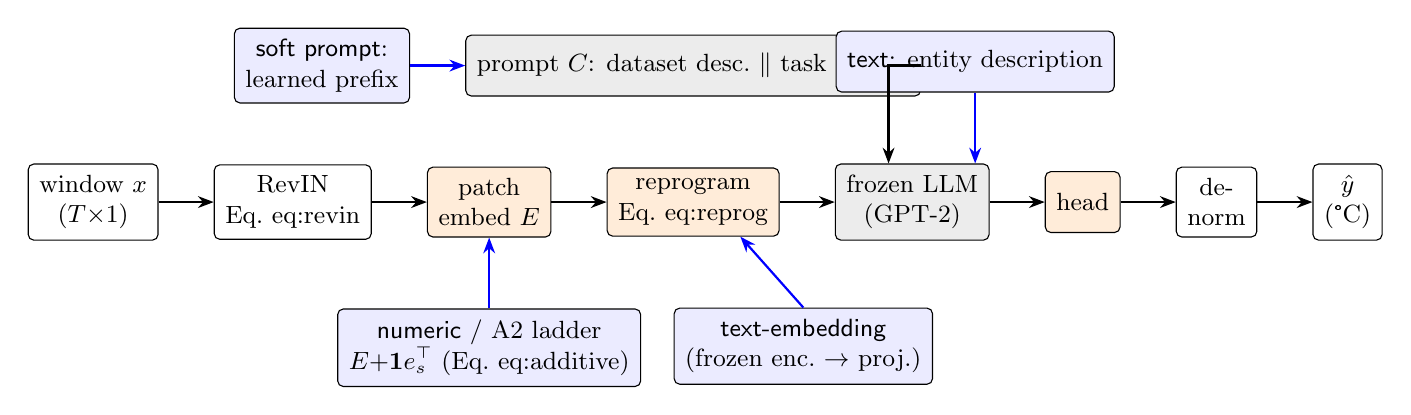
\begin{tikzpicture}[
  font=\small,
  box/.style={draw, rounded corners=2pt, minimum height=2.2em, inner sep=4pt, align=center},
  idbox/.style={box, fill=blue!8},
  frozen/.style={box, fill=gray!15},
  train/.style={box, fill=orange!15},
  arr/.style={-{Stealth[length=2mm]}, thick},
  node distance=5mm and 7mm]

\node[box] (x) {window $x$\\$(T{\times}1)$};
\node[box, right=of x] (revin) {RevIN\\Eq.~\eqref{eq:revin}};
\node[train, right=of revin] (patch) {patch\\embed $E$};
\node[train, right=of patch] (reprog) {reprogram\\Eq.~\eqref{eq:reprog}};
\node[frozen, right=of reprog] (llm) {frozen LLM\\(GPT-2)};
\node[train, right=of llm] (head) {head};
\node[box, right=of head] (denorm) {de-\\norm};
\node[box, right=of denorm] (yhat) {$\hat{y}$\\(°C)};

\node[idbox, below=9mm of patch] (numeric) {\textsf{numeric} / A2 ladder\\$E{+}\mathbf{1}e_s^{\top}$ (Eq.~\eqref{eq:additive})};
\node[idbox, below=9mm of reprog, xshift=14mm] (textemb) {\textsf{text-embedding}\\(frozen enc.\ $\to$ proj.)};

\node[frozen, above=9mm of reprog] (prompt) {prompt $C$: dataset desc.\ $\|$ task $\|$ stats};
\node[idbox, above=9mm of llm, xshift=8mm] (textid) {\textsf{text}: entity description};
\node[idbox, left=7mm of prompt] (soft) {\textsf{soft prompt}:\\learned prefix};

\draw[arr] (x) -- (revin);
\draw[arr] (revin) -- (patch);
\draw[arr] (patch) -- (reprog);
\draw[arr] (reprog) -- (llm);
\draw[arr] (llm) -- (head);
\draw[arr] (head) -- (denorm);
\draw[arr] (denorm) -- (yhat);
\draw[arr, blue] (numeric) -- (patch);
\draw[arr, blue] (textemb.north) -- ([xshift=6mm]reprog.south);
\draw[arr] (prompt.east) -| ([xshift=-3mm]llm.north);
\draw[arr, blue] (textid) -- ([xshift=8mm]llm.north);
\draw[arr, blue] (soft) -- (prompt);
\end{tikzpicture}
\caption{Framework. Gray blocks are frozen, orange blocks train, and the four blue
blocks are the identity-injection schemes under comparison (the study's axis):
\textsf{numeric}/A2 adds a station vector to the patch embeddings after RevIN,
\textsf{text-embedding} injects a projected frozen text encoding at the same site,
\textsf{text} inserts a per-station description into the prompt, and \textsf{soft
prompt} prepends learned per-station tokens. \textsf{none} removes all blue blocks
and reproduces official Time-LLM byte-for-byte. RevIN erases per-window level and
scale (Section~\ref{sec:method}), which is why every injection site sits downstream
of it.}
\label{fig:framework}
\end{figure*}

Figure~\ref{fig:framework} places the four schemes on one diagram: two injection
positions (prompt pathway vs.\ additive at the patch embeddings), two
representation sources (text vs.\ learned), every site downstream of RevIN, and
the backbone frozen throughout.

\subsection{Pipeline}

One matrix entry expands cells (dataset $\times$ scheme $\times$ sub-variant
$\times$ seed) into a shared pipeline: every scheme trains under the SAME fixed
backbone configuration (Section~\ref{sec:setup}) with validation early stopping
(patience 10), and the best-validation epoch's checkpoint is evaluated once.
Metrics are reported in scaler space and in physical units (denormalized RMSE,
°C). The same pipeline trains the classical baselines (LSTM, PatchTST, DLinear),
which keeps cross-family numbers comparable. The pipeline also supports a
matched-budget Ray~Tune HPO mode (ASHA over
$\{lr\}\times\{d_{\mathrm{model}}\}\times\{d_{\mathrm{ff}}\}\times\{\mathit{llm\_layers}\}$),
which we reserve for a sensitivity pass on the flagship cells.

\section{Experimental Setup}
\label{sec:setup}

\textbf{Datasets.} Three Swiss river water-temperature collections (daily means,
per-entity 80/20 split): \swiss{} (28 stations, 1990--2020, entity-rich; measured
warming trend $+0.268$\,°C/decade by Theil--Sen, consistent with the national
literature value $+0.33\pm0.03$~\cite{michel2020}), \swissb{}, and \swissc{}.
Authored prompts contain only facts traceable to the data or cited literature, with
per-phrase provenance kept in the repository.

\textbf{Protocol: fixed configuration, faithful to the original.} The original
Time-LLM paper reports \emph{fixed} per-dataset configurations (its
Appendix~B.4, Table~9; B.1: ``We mainly follow the experimental configurations in
(Wu et al., 2023)'') and describes no hyper-parameter search; its released code
applies validation early stopping (patience 10) but no tuning. We adopt the same
discipline: every scheme trains under ONE fixed backbone configuration --- the
canonical Time-LLM values ($d_{\mathrm{model}}{=}32$, $d_{\mathrm{ff}}{=}128$,
$n_{\mathrm{heads}}{=}8$, 6 GPT-2 layers), batch 32, horizon 7 days, patch 16/8
shared with PatchTST, 30 epochs with patience-10 early stopping, bf16 mixed
precision exactly as the official code --- with a single evidence-based
deviation, $lr{=}10^{-3}$ instead of the canonical $10^{-2}$, selected once by a
100-epoch diagnostic on the \textsf{none} baseline (validation denorm RMSE 1.746
vs.\ 1.811) BEFORE any scheme comparison, then frozen for all schemes. Because
every scheme shares this configuration, the comparison is internally matched;
identity-specific parameters are fixed too (soft-prompt length 8; the numeric
identity width is structurally tied to $d_{\mathrm{model}}$). Seed 2026 across
all model families (single seed until the design freezes; a multi-seed pass is
affordable under this protocol and follows). The Time-LLM port reproduces the
official repository bit-exactly on ETTh1 (per-epoch losses identical; Test MSE
0.3908 / MAE 0.4159). A matched-budget HPO sensitivity pass on the flagship cells
is planned to confirm the fixed-configuration conclusions. Comparisons never mix
precision, prompt file, or protocol; such changes deploy only at tier
boundaries.

\textbf{Arms.} Both a \emph{promptfix} arm (authored Swiss description) and an
\emph{ETT-control} arm (official electricity description, everything else equal)
run the full grid, so the value of a domain-correct description is itself measured
at matched budget.

\section{Results}
\label{sec:results}

\subsection{What identity is worth: classical reference points}

\begin{table}[t]
\caption{Identity effects in classical models on \swiss{} (benchmark round;
one-hot identifiers).}
\label{tab:classical}
\begin{tabular}{@{}lll@{}}
\toprule
model & identifier effect & reading \\
\midrule
LSTM & $-56\%$ RMSE ($\approx$1.17\,°C) & identity dominates architecture \\
PatchTST & $-7.5\%$ & attenuated by patching \\
DLinear & $\pm0.25\%$ & linear model cannot exploit it \\
\bottomrule
\end{tabular}
\end{table}

Table~\ref{tab:classical} sets the scale: identity is worth more than most
architecture choices in this domain, which makes the frozen-LLM question
non-trivial.

\subsection{Scheme comparison on Time-LLM: single-seed anchors}

\begin{table}[t]
\caption{Time-LLM identity schemes on \swiss{}: single-seed sanity ANCHORS from
the \emph{completed} harness runs of 2026-08-02/03 (seed 2026, the canonical
Time-LLM hyper-parameters, no HPO; every number is a finished run archived in the
repository). The harness reported scaler-space Test MSE only; the running matched
grid of Table~\ref{tab:main} re-measures all schemes and reports physical-unit
denormalized RMSE (°C), the same convention as our ICPR 2026 paper, which is the
metric the paper's headline claims will use. These anchors are kept because their
\emph{directions} motivated the study design.}
\label{tab:anchors}
\begin{tabular}{@{}lll@{}}
\toprule
scheme & Test MSE & $\Delta$ vs.\ \textsf{none} \\
\midrule
\textsf{none} & 0.014177 & --- \\
\textsf{text} (entity description) & 0.014485 & $+2.2\%$ \\
\textsf{numeric} (learnable) & 0.011433 & $\mathbf{-19.4\%}$ \\
\textsf{random} (fixed, matched dim) & 0.011569 & $-18.4\%$ \\
\bottomrule
\end{tabular}
\end{table}

Two observations drive the paper. First, the additive numeric pathway carries a
large gain while the prompt-text pathway carries none, \emph{through the same
frozen backbone} --- the injection position matters more than the information.
Second, a capacity-matched random identity recovers 95\% of the learnable gain,
reproducing in the LLM setting the signature Li et al.~\cite{li2022random} found
for classical hydrological models: distinctness, not content.

A cross-domain check reinforces that identity is not a free regularizer: the same
numeric scheme that helps entity-rich \swiss{} ($-17.6\%$ in the cross-check run)
\emph{hurts} ETTh1 ($+2.3\%$), whose channels are sensor variables of one site
rather than distinct entities.

\subsection{Main matched grid}
\label{sec:main}

\begin{table}[t]
\caption{Main results: injection schemes under the fixed shared configuration
(Section~\ref{sec:setup}), frozen backbone, seed 2026. Physical-unit denormalized RMSE (°C) with scaler-space MSE in
parentheses.
% [orig 2026-08-16] \inprogress{chains 11907034--11907039; phase order: none -> numeric -> text/soft/text-embedding}
All fifteen cells complete.}
\label{tab:main}
\begin{tabular}{@{}lccc@{}}
\toprule
scheme & \swiss{} & \swissb{} & \swissc{} \\
\midrule
% [orig 2026-08-16 placeholders]
% \textsf{none} & \inprogress{running} & --- & --- \\
% \textsf{numeric} & --- & --- & --- \\
% \textsf{text} & --- & n/a$^{\dagger}$ & n/a$^{\dagger}$ \\
% \textsf{soft prompt} & --- & --- & --- \\
% \textsf{text-embedding} & --- & n/a$^{\dagger}$ & n/a$^{\dagger}$ \\
\textsf{none} & 1.8658 & 1.8360 & 1.9407 \\
\textsf{numeric} & \textbf{1.5833} ($-15.1\%$) & \textbf{1.7203} ($-6.3\%$) & 1.9690$^{\ddagger}$ \\
\textsf{text} & 1.8537 & 1.8253 & 1.9393 \\
\textsf{soft prompt} & 1.8786 & 1.8372 & 1.9357 \\
\textsf{text-embedding} & 1.8748 & 1.8338 & 1.9207 \\
\bottomrule
\multicolumn{4}{@{}p{0.94\linewidth}@{}}{\footnotesize $^{\ddagger}$\swissc{}
numeric is inside the measured run-to-run noise band: an identical-configuration
restart gave 1.8861 ($-2.8\%$), a ${\approx}4\%$ spread, so the honest \swissc{}
statement is ``no reliable effect,'' not ``hurts.'' The numeric embedding width was
grid-selected over $\{8,16,32\}$ per dataset (winners 16/32/8); a $\{1,2,4,8\}$
probe on \swissc{} confirmed no width below 8 helps.}
\end{tabular}
\end{table}

% [orig 2026-08-16] Table~\ref{tab:main} is the paper's centerpiece and is being produced by the two
% cluster chains (promptfix and ETT-control arms; about 27 hours per cell, 24-hour
% dependency-chained segments). The ETT-control twin of Table~\ref{tab:main}
% isolates the dataset-description value.
Table~\ref{tab:main} is complete (all fifteen cells measured under the fixed
protocol). The pattern is uniform: the additive numeric pathway is the only scheme
that carries a significant gain (per-station Wilcoxon, Section~\ref{sec:analysis}:
$p{=}1.2{\times}10^{-4}$ on \swiss{}), every language-pathway scheme sits within
$\pm1\%$ of \textsf{none} --- and \textsf{soft prompt} and \textsf{text-embedding}
are significantly \emph{worse} than \textsf{none} ($p{<}5{\times}10^{-3}$). The
numeric gain itself scales with entity richness ($-15.1\%\rightarrow-6.3\%%
\rightarrow{\approx}0$ across the three collections).

\section{Ablations and Supplementary Experiments}
\label{sec:ablations}

\textbf{Injection position vs.\ normalization (done, PatchTST).} Identity
concatenated to the \emph{input} is erased by instance normalization ($+30$--$85\%$
error); the same identity added after patch embedding survives. This fixes the
additive site downstream of RevIN and confirms the erasure argument of
Section~\ref{sec:method} empirically.

% [orig 2026-08-16] Distinguisher vs. content was "arms implemented; runs queued" with the
% pre-registered readouts spelled out; the ladder has now RUN. Original text:
% The prompt ladder none -> symbol (five-letter consonant codes; pure distinctness,
% no ordinal leak) -> minimal -> shuffled (authored words, order destroyed) -> default
% -> stats (adds train-only per-station statistics) decomposes the text pathway.
% Pre-registered readouts: shuffled ~= default implies the prompt acts as a
% distinctness token, not as language; symbol ~= default implies content is
% irrelevant. Per the study design the ladder runs with the backbone frozen; the
% fine-tuned repeat is a follow-up tier.
\textbf{Distinguisher vs.\ content (done, frozen backbone, \swiss{}).} The
pre-registered prompt ladder ran: \textsf{default} 1.8537, \textsf{shuffled}
(authored words deranged between stations) 1.8628, \textsf{symbol} (meaningless
codes) 1.8657, \textsf{minimal} 1.8835, vs.\ \textsf{none} 1.8658. All arms are
within $\pm1\%$ of \textsf{none} and \textsf{default}$\,\approx\,$%
\textsf{shuffled}$\,\approx\,$\textsf{symbol}$\,\approx\,$\textsf{none}
(pairwise n.s.). The frozen language pathway is deaf to the station text
\emph{entirely}: neither content (correct vs.\ deranged indistinguishable) nor
even bare distinctness (\textsf{symbol} vs.\ \textsf{none}) reaches the
forecast. This sharpens the pre-registered readout: the prompt does not even act
as a distinctness token.

% [orig 2026-08-16] Backbone depth (inside the running grid). The official code default
% truncates GPT-2 to 6 layers while the paper reports full depth 2.7% better;
% llm_layers in {3,6,12} is an HPO dimension of every cell, so validation decides.
\textbf{Backbone depth.} The fixed protocol pins $\mathit{llm\_layers}{=}6$ (the
official code default); the backbone ablation below additionally measures depth 0.

\textbf{Optimizer diagnostic (done).} Both the canonical $lr=10^{-2}$ and
$10^{-3}$ converge by epoch ${\approx}8$ under early stopping on
\swiss{}$\times$\textsf{none}; $10^{-3}$ wins validation (denorm RMSE 1.746 vs.\
1.811), so both stay in the HPO grid rather than being fixed by convention.

\textbf{Is the LLM doing anything? (done, \swiss{}).} A three-arm backbone
ablation holds the entire trainable path fixed (52.7M reprogramming + head
parameters, identical in every arm) and swaps only the frozen stack:

\begin{table}[t]
\caption{Backbone ablation on \swiss{} (fixed protocol, seed 2026, denorm RMSE
°C). Trainable parameters identical across arms; only the frozen stack differs.
Extension to \swissb{}/\swissc{} \inprogress{running, jobs 12435489/12435490}.}
\label{tab:backbone}
\begin{tabular}{@{}lccc@{}}
\toprule
frozen backbone & \textsf{none} & \textsf{numeric} & gain \\
\midrule
pretrained GPT-2 (6 blocks) & 1.8658 & 1.6471 & $-11.7\%$ \\
random-init GPT-2 (6 blocks) & 1.8559 & \textbf{1.5241} & $-17.9\%$ \\
no LLM (0 blocks) & 1.8586 & 1.5652 & $-15.8\%$ \\
\bottomrule
\end{tabular}
\end{table}

All three \textsf{none} cells agree to $0.5\%$ (pairwise n.s.) --- deleting the
frozen stack costs nothing on the base task and trains $3.5\times$ faster. The
identity gain survives every backbone (all $p{\le}2.8{\times}10^{-6}$ vs.\
\textsf{none}), so it lives in the trainable path, not in the language model.
This reproduces Tan et al.~\cite{tan2024llmuseful} on hydrological data and
extends it with the identity axis they did not test.

\textbf{A small LSTM through the same pipeline (done).} Under the identical
protocol (same splits, loaders, metric, 30 epochs, no tuning), a plain LSTM beats
the 134M-parameter frozen-LLM system in \emph{every} cell: \textsf{none}
1.6371/1.6736/1.5645 and \textsf{numeric} 1.3061/1.4043/1.3302 on
\swiss{}/\swissb{}/\swissc{}, i.e.\ identity gains of $-20.2\%/-16.1\%/-15.0\%$
that are uniform across collections where Time-LLM's decay to zero. An HPO
companion (10 Ray trials per cell) moves no cell by more than a few percent and
reproduces our ICPR-line result (1.2889 on \swiss{} numeric vs.\ the earlier
$1.294\pm0.007$), ruling out tuning as the explanation for the gap. Notably the
LSTM exploits a ${\sim}16$-dimensional identity even on \swissc{}, where the
frozen Time-LLM can use none.

\textbf{Unfreezing: the LoRA $2{\times}2$ (done, \swiss{}).} The decisive test
of whether pretrained language knowledge can serve the text pathway at all:

\begin{table}[t]
\caption{LoRA $2{\times}2$ on \swiss{} (r=4, $\alpha$=8 on \texttt{c\_attn};
73.7K adapter parameters; fixed protocol, seed 2026, denorm RMSE °C).
\inprogress{\swissb{}/\swissc{} extension running.}}
\label{tab:lora}
\begin{tabular}{@{}llccc@{}}
\toprule
backbone & tuning & \textsf{none} & \textsf{text} & \textsf{numeric} \\
\midrule
pretrained & frozen & 1.8658 & 1.8537 & 1.6471 \\
pretrained & LoRA & 1.8834 & \textbf{1.5442} & 1.6137 \\
random-init & frozen & 1.8559 & 1.8511 & 1.5241 \\
random-init & LoRA & 1.8534 & 1.8508 & 1.5142 \\
\bottomrule
\end{tabular}
\end{table}

The four corners separate cleanly. LoRA wakes the text pathway \emph{only} on the
pretrained backbone ($1.8537\rightarrow1.5442$, $-17.2\%$ vs.\ \textsf{none},
$p{=}7.5{\times}10^{-8}$) --- on par with the numeric scheme, from 73.7K adapter
parameters. The random-initialized control shows no rescue (1.8508, a $\sim$1\%
effect an order of magnitude smaller), so the rescue is not generic trainable
capacity; it requires the pretrained weights. Two specificity controls hold: LoRA
on \textsf{none} is significantly \emph{worse} (adapters with no information
channel add noise), and LoRA barely moves \textsf{numeric} (the additive channel
never needed the LLM). Together with the backbone ablation this yields the paper's
arc: \emph{the frozen protocol leaves the language model dead weight; a minimal
adaptation turns its pretraining into a working entity-identity channel.}

\textbf{Queued controls.} A2 ladder (random / one-hot / sinusoidal / coordinates);
norm-range 2$\times$2 (min-max vs.\ z-score $\times$ identity); GPT4TS as the
no-prompt negative control (implemented); Chronos zero-shot; identity $\times$
trainability 2$\times$2 --- deferred by design so the frozen scheme comparison
lands first.

\section{Analysis Plan (pre-registered)}
\label{sec:analysis}

The battery below is fixed \emph{before} the grid lands, and each item states its
decision rule.

\textbf{Significance protocol (executed).} Following our ICPR benchmark practice,
every comparison against \textsf{none} is tested with a Wilcoxon signed-rank test
over paired \emph{per-station} test errors (n = 28/63/15 stations), computed from
the saved best-checkpoint predictions in °C. All headline claims above carry these
$p$-values: numeric gains $p\le2.2{\times}10^{-2}$ (down to $7.5{\times}10^{-9}$
across backbones), the LoRA text wake-up $p{=}7.5{\times}10^{-8}$, soft-prompt and
text-embedding significantly worse than \textsf{none} ($p{<}5{\times}10^{-3}$),
and the backbone-equivalence claims correctly non-significant.

\begin{enumerate}
\item \textbf{Main-effect table.} Scheme vs.\ \textsf{none} per dataset at matched
budget, in °C; single-seed status stated explicitly until the multi-seed pass.
\item \textbf{Distinctness vs.\ content.} Apply the ladder inequalities of
Section~\ref{sec:ablations}; every branch yields a publishable statement, including
the null.
\item \textbf{Capacity-matched controls.} If \textsf{random}$\,\approx\,$%
\textsf{numeric} at matched dimension in the HPO-matched grid, the mechanism claim
is distinctness, and the bridge to Li et al.~\cite{li2022random} becomes the
discussion anchor.
\item \textbf{Linear probes.} Decode station identity from patch representations
before and after injection with a Hewitt--Liang selectivity control; the claim
``identity reaches the representation'' must survive the control.
\item \textbf{Attention and geometry.} Prompt-to-patch attention mass and t-SNE of
per-station mean representations; falsifiable statement: injection increases
between-station separation (silhouette) without degrading temporal structure.
\item \textbf{Knowledge vs.\ fitting.} Cross-station window transplants and
inference-time prompt swaps decide whether any text gain is semantic or
surface-statistical.
\item \textbf{Discrepancy protocol.} If the matched grid reverses an anchor
direction, resolved per-cell configs are audited before any scientific claim; no
number enters the paper without its results file and config hash.
\end{enumerate}

\section{Limitations and Future Work}
Single seed until the design freezes; one country and one variable; station
descriptions currently exist for \swiss{} only; LLaMA-scale backbones pending
cluster time; the ETT-control arm controls the dataset description, not the task
instructions.

\textbf{Further models (named).} The scheme comparison extends beyond Time-LLM to
the other reprogramming and LLM-based forecasters already ported to the same entry
and pipeline: GPT4TS~\cite{zhou2023onefitsall} (implemented; the no-prompt negative
control), TEMPO~\cite{cao2024tempo} (implemented; decomposition variant),
AutoTimes~\cite{liu2024autotimes} (implemented; autoregressive time tokens),
CALF (cross-modal dual branch; port planned), and UniTime (the second
native-text backbone; planned). Backbone sensitivity within Time-LLM covers GPT-2,
BERT, and LLaMA-7B (weights staged on the cluster), and Chronos-2 serves as a
zero-shot foundation-model control without any learned entity pathway.

\textbf{Further data (named).} Beyond the three Swiss water-temperature
collections: CAMELS-CH-Chem (86 hourly Swiss stations; a station-alignment
leakage check against our 28 stations precedes any use), and the cross-domain
entity-strength ladder already wired in the repository --- traffic (862 sensors,
strong entities), electricity (321 clients), and ETTh1 (sensor variables of one
site, the deliberately weak-entity control) --- which turns the domain-dependence
observation of Section~\ref{sec:results} into a systematic axis.

\section{Conclusion}
% [orig 2026-08-16] \inprogress{written after the matched grid lands; the candidate storyline ---
% injection position dominates representation source, and distinctness carries the
% gain --- is falsifiable by Tables~\ref{tab:main} and the ladder.}
We compared five ways of telling a reprogrammed, frozen time series LLM
\emph{which station} it is forecasting, on three Swiss river water temperature
collections under one fixed protocol. The comparison resolves cleanly: injection
position dominates representation source. The additive numeric pathway carries the
only significant gain, and the frozen language pathway is deaf --- correct
descriptions, deranged descriptions, and meaningless codes are indistinguishable
from no text at all, with soft prompts and text embeddings significantly worse
than nothing. Backbone ablations then sharpen the diagnosis: random weights or no
frozen stack at all match the pretrained backbone everywhere, and a plain LSTM
through the same pipeline beats the 134M-parameter system in every cell --- under
the original frozen protocol the language model is dead weight. The turn is that a
74K-parameter LoRA adapter recovers the language pathway, and only on the
pretrained backbone: text identity then matches numeric identity
($p{=}7.5{\times}10^{-8}$), while the random-initialized control gains nothing.
Pretrained language knowledge is neither useless nor freely available --- it is
locked behind the frozen interface, and a minimal adaptation opens it. Because a
station's description, unlike its embedding row, exists before any data is
collected, this opens a concrete path we are pursuing next: cold-start forecasting
for ungauged stations.

\bibliographystyle{ACM-Reference-Format}
\bibliography{references}

\end{document}
